\documentclass[14pt,aspectratio=169]{beamer}

\usepackage{pgfpages}
\usepackage{fancyvrb}
\usepackage{pgfplots}

\usepackage{minted}
\usemintedstyle{tango}

\usepackage{amsfonts}

\usepackage{moresize}
\usepackage{anyfontsize}

\usepackage{tikz}
\usetikzlibrary{arrows,shapes}
\usetikzlibrary{arrows.meta}

\tikzstyle{process}=[rectangle, draw, thick, text width=5em, text centered, minimum height=2.5em, fill=gray!40]
\tikzstyle{entity}=[rounded rectangle, draw, thick, text width=5em, text centered, minimum height=1.5em, fill=gray!40]

\usetheme{auriga}
\usecolortheme{auriga}

\setbeamercolor{background canvas}{bg=lightgray}

% define some colors for a consistent theme across slides
\definecolor{red}{RGB}{181, 23, 0}
\definecolor{blue}{RGB}{0, 118, 186}
\definecolor{gray}{RGB}{146, 146, 146}

\title{Discrete Structures: \\ Basics of Mathematics and Programming}

\author{{\bf Gregory M. Kapfhammer}}

\institute[shortinst]{{\bf Department of Computer Science, Allegheny College}}

\begin{document}

{
  \setbeamercolor{page number in head/foot}{fg=background canvas.bg}
  \begin{frame}
    \titlepage
  \end{frame}
}

%% Slide
%
\begin{frame}{Technical Question}
  %
  \begin{center}
    %
    {\large How do I connect mathematical terminology (e.g., {\em mapping}, {\em
      function}, {\em number}, {\em sequence}, and {\em set}), to the
      implementation of Python programs that declare and call functions and declare
    and manipulate variables?}
    %
  \end{center}
  %
  \vspace{2ex}
  %
  \begin{center}
    %
    \small Let's learn more about how the use of precise mathematical terms and
    concepts helps to effectively communicate and perform programming tasks!
    %
  \end{center}
  %
\end{frame}

% Slide
%
\begin{frame}{Discrete Structures = Math + Programming}
%
  \begin{itemize}
    %
    \item Discrete mathematics: symbols, character strings, truth values,
      objects, and collections of these entities
      %
    \item Specifying and designing a computer program
      \begin{itemize}
        \item Describe input, output, and internal objects
        \item Use the vocabulary of discrete mathematics
        \item Implement and test the program in a language
      \end{itemize}
      %
    \item Our goal: implement a program $P$ meets a specification $S$
      %
  \end{itemize}
%
\end{frame}

% Slide
%
\begin{frame}{Specifying a Program that Analyzes Web Pages}
  %
  \begin{itemize}
    %
    \item Informal specification: Read two web pages and then find and output
      all of the URLs that appear in them both
      %
    \item Different approaches to implementing this program
      %
      \begin{itemize}
        %
        \item Informal and intuitive specification
          %
        \item Precise mathematical specification
          %
        \item Which one is shorter? ... clearer? ... unambiguous?
      \end{itemize}
      %
    \item Mathematics helps us to implement a program that is correct,
      efficient, documented, and maintainable!
      %
  \end{itemize}
  %
\end{frame}

% Slide
%
\begin{frame}{Programs, Data, and Mathematical Objects}
  %
  \begin{itemize}
    %
    \item Our goal: Jump to different levels of abstraction (e.g., high-level
      versus low-level) when we create programs
      %
      \vspace*{-.2in}
      %
    \item What {\em is} a computer program?
      %
      \begin{itemize}
        %
        \item Informal or intuitive specification
          %
        \item Precise discrete mathematical specification
          %
        \item Realization of a specification in Python program
          %
        \item Bits packaged into bytes and words stored on a disk
          %
        \item A process in execution on a CPU and stored in memory
          %
      \end{itemize}
      %
      \vspace*{-.2in}
      %
    \item It is ``natural'' (and fun!) to jump from a discrete mathematical
      specification to a Python program
      %
  \end{itemize}
  %
\end{frame}

% Slide
%
\begin{frame}{Using Python to Explore Discrete Structures}
  %
  \begin{itemize}
    %
    \item Discrete structures support precise programming
      %
    \item Benefits of using Python to explore discrete structures
      %
      \begin{itemize}
        %
        \item Modern language with exceptional package support
          %
        \item Clean syntax and semantics that is easy to learn
          %
        \item Out-of-the-box support for many discrete structures
          %
      \end{itemize}
      %
    \item Download Python and start programming by visiting
      \url{https://www.python.org/}
      %
  \end{itemize}
  %
\end{frame}

% Slide
%
\begin{frame}{A First Look at the Python Language}
  %
  \begin{itemize}
    %
    \item Python is an exceptional programming language supported by an
      ultra-exceptional community
      %
      \vspace*{-.15in}
      %
    \item How can we describe the Python language?
      %
      \begin{itemize}
        %
        \item Scripting language
          %
        \item Object-oriented language
          %
        \item Function-oriented language
          %
        \item High-level language
          %
      \end{itemize}
      %
      \vspace*{-.15in}
      %
    \item VSCode provides support for Python through syntax highlighting, source
      code processting, linting, and testing
      %
  \end{itemize}
  %
\end{frame}

% Slide
%
\begin{frame}[fragile]
  \frametitle{Using Python to Find a Name in a File}
  \normalsize
  \hspace*{-.65in}
  \begin{minipage}{6in}
    \vspace*{.25in}
    \begin{minted}[mathescape, numbersep=5pt, fontsize=\large]{python}
    file = open("names")
    for line in file:
      if line.startswith("John")
        print(line)
    \end{minted}
  \end{minipage}
  \vspace*{.25in}
  \begin{center}
    %
    \normalsize \noindent Can you explain the behavior of this program segment? \\
    \normalsize \noindent How is this different than a full-fledged Python program? \\
    \normalsize \noindent What is the purpose of the {\tt line.startswith} function? \\
    %
  \end{center}
  %
\end{frame}

% Slide
%
\begin{frame}[fragile]
  \frametitle{Using Python to Find a Name in a File}
  \normalsize
  \hspace*{-.65in}
  \begin{minipage}{6in}
    \vspace*{.25in}
    \begin{minted}[mathescape, numbersep=5pt, fontsize=\large]{python}
    file = open("emails")
    for line in file:
      name, email = line.split(",")
      if name = "John Davis":
        print(email)
    \end{minted}
  \end{minipage}
  \vspace*{.25in}
  \begin{center}
    %
    \normalsize \noindent Can you explain the behavior of this program segment? \\
    \normalsize \noindent What type of data are {\tt name} and {\tt email}? \\
    \normalsize \noindent What is the purpose of the {\tt line.split} function? \\
    %
  \end{center}
  %
\end{frame}

% Slide
%
\begin{frame}[fragile]
  \frametitle{Using Python to Average Numerical Values}
  \hspace*{-.6in}
  \begin{minipage}{6in}
    \begin{minted}[mathescape, numbersep=5pt, fontsize=\large]{python}
    sum = 0
    count = 0
    file = open("observations")
    for line in file:
      n = int(line)
      sum += n
      count += 1
    print(sum/count)
    \end{minted}
  \end{minipage}
\end{frame}

% Slide
%
\begin{frame}{Python Programming Retrospective}
  %
  \begin{itemize}
    %
    \item Intuitively read the code segments to grasp their behavior
      %
      \vspace*{-.15in}
      %
    \item Key components of the Python programming segments
      %
      \begin{itemize}
        %
        \item Function calls
          %
        \item Assignment statements
          %
        \item Iteration constructs
          %
        \item Conditional logic
          %
        \item Variable creation
          %
        \item Variable computations
          %
        \item Variable output
          %
      \end{itemize}
      %
      \vspace*{-.2in}
      %
    \item Make sure that you can find all of these components!
      %
  \end{itemize}
  %
\end{frame}



% Slide
%
\begin{frame}{Useful Mathematical Terminology}
  %
  \begin{itemize}
    %
    \item To be clear and succinct, we use mathematical terminology as a
      vocabulary for talking about Python programs
      %
      \vspace*{-.15in}
      %
    \item What are mathematical terms that aid programming?
      %
      \begin{itemize}
        %
        \item {\bf Set}: an unordered collection of different entities
          %
        \item {\bf Sequence}: an ordered collection of entities
          %
        \item {\bf Relation}: a set that relates pairs of things with each other
          %
        \item {\bf Mapping}: a set of ordered pairs in which no two first
          elements are the same (sometimes called a ``function'' in mathematics)
          %
      \end{itemize}
      %
      \vspace*{-.2in}
      %
    \item Can you find these mathematical concepts in the Python programs?
      What is a file? What does iteration process?
      %
  \end{itemize}
  %
\end{frame}

% Slide
%
\begin{frame}{Properties of Integer Addition}
  %
  \vspace*{-.15in}
  %
  \begin{itemize}
    %
    \item The average computation program processes integer values that are
      governed by mathematical rules
      %
      \vspace*{-.15in}
      %
    \item Precisely define the set of observations: $O = \{ o_i : o_i \in
      \mathbb{Z}\}$
      %
      \vspace*{-.15in}
      %
    \item Two properties of integer addition
      %
      \begin{itemize}
        %
        \item {\bf Associative}: $(a + b) + c = a + (b + c), \forall a, b, c \in
          \mathbb{Z}$
          %
        \item {\bf Commutative}: $a + b = b + a, \forall a, b \in \mathbb{Z}$
          %
      \end{itemize}
      %
      \vspace*{-.2in}
      %
    \item Wait, is the collection of observations a set? No, not if it contained
      recorded temperature values! It can have repeated items, which means it is
      a {\bf multiset}.
      %
  \end{itemize}
  %
\end{frame}

%% Slide
%
\begin{frame}{Expressing Average Computation with Multisets}
  %
  \vspace*{-.5in}
  \begin{center}
  \fontsize{20}{30}\selectfont
    \begin{equation*}
     O = \{\!\{o_1, \ldots, o_n\}\!\}
    \end{equation*}
    \begin{equation*}
      S = \sum_{o_i \in O} o_i
    \end{equation*}
    \begin{equation*}
      A = \frac{S}{|O|}
    \end{equation*}
  \end{center}
  %
  \vspace{2ex}
  %
  \begin{center}
    %
    \small What is the meaning of $o_i \in O$? Where does this exist in Python code?
    %
  \end{center}
  %
\end{frame}

%% Slide
%
\begin{frame}{Expressing Average Computation with Multisets}
  %
  \vspace*{-.5in}
  \begin{center}
  \fontsize{20}{30}\selectfont
    \begin{equation*}
     O = \{\!\{o_1, \ldots, o_n\}\!\}
    \end{equation*}
    \begin{equation*}
      S = \sum_{i=1}^{n} o_i \in O
    \end{equation*}
    \begin{equation*}
      A = \frac{S}{n}
    \end{equation*}
  \end{center}
  %
  \vspace{2ex}
  %
  \begin{center}
    %
    \small What is the meaning of $\sum_{i=1}^{n} o_i$? Where does this exist in Python code?
    %
  \end{center}
  %
\end{frame}


% Slide
%
\begin{frame}{Summary of the ``Abstraction Jumping''}
  %
  \begin{itemize}
    %
    \item What is the connection between the discrete mathematical structures
      and the Python programs?
      %
      \vspace*{-.15in}
      %
    \item Connections between discrete mathematics and Python
      %
      \begin{itemize}
        %
        \item {\bf Generic file}: a sequence of sequences
          %
        \item {\bf Names in the file}: a set of strings
          %
        \item {\bf Emails in the file}: a set of ordered pairs forming a
          relation
          %
        \item {\bf Temperatures in the file}: a multiset of integers
          %
      \end{itemize}
      %
      \vspace*{-.2in}
      %
    \item When might the emails in the file be a mapping? When might the
      temperatures in the file be a sequence?
      %
  \end{itemize}
  %
\end{frame}

% Slide
%
\begin{frame}{Analyzing and Visualizing Temperature Values}
  %
  \begin{figure}
    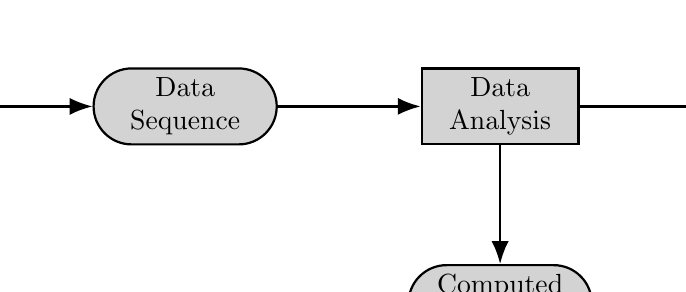
\begin{tikzpicture}[node distance=4cm, auto,>=latex', thick]
      %
      \path[use as bounding box] (2,1) rectangle (10,-2);
      %
      % Sensor* --> Data Sequence*
      %
      \path[->] node[process, font=\large] (sensor) {Sensor};
      \path[->] node[entity, right of=sensor, align=center] (values) {Data \\ Sequence};
      \path [draw, thick, -{>[scale=1.25]}, >=Latex] (sensor.east) -- (values.west);
      %
      % Data Sequence --> Data Analysis*
      %
      \path[->] node[process, right of=values, align=center] (analyze) {Data \\ Analysis};
      \path [draw, thick, -{>[scale=1.25]}, >=Latex] (values.east) -- (analyze.west);
      %
      % Data Analysis --> Computed Average*
      %
      \path[->] node[entity, below of=analyze, align=center, yshift=1.5cm] (average) {Computed \\ Average};
      \path [draw, thick, -{>[scale=1.25]}, >=Latex] (analyze.south) -- (average.north);
      %
      % Data Analysis --> Data Visualization*
      %
      \path[->] node[entity, right of=analyze, align=center] (graph) {Data \\ Graph};
      \path [draw, thick, -{>[scale=1.25]}, >=Latex] (analyze.east) -- (graph.west);
      %
    \end{tikzpicture}
    %
    \vspace*{.6in}
    \begin{center}
      %
      \normalsize
      %
      \noindent Why should we view the sensor's output as a sequence? \\
      What is the data type for the computed average? \\
      How would we visualize a sequence of temperature values?
      %
    \end{center}
    %
  \end{figure}
  %
\end{frame}

% Slide
%
\begin{frame}{Further Connecting Mathematics and Python}
  %
  \begin{itemize}
    %
    \item Variables and their associated types exist in both discrete
      mathematics and in Python programs
      %
      \vspace*{-.15in}
      %
    \item Connecting mathematical variables to Python variables
      %
      \begin{itemize}
        %
        \item $a \in \mathbb{Z}$ means that $a$ is an integer value in Python
          %
        \item $a \in \mathbb{R}$ means that $a$ is a floating point value in
          Python
          %
        \item Python variables have descriptive names like {\tt child\_count}
          %
        \item Python variables can also store character strings like {\tt
          "radio"}
          %
      \end{itemize}
      %
      \vspace*{-.2in}
      %
    \item Python variables have practical limitations not faced by
      mathematical ones! What are they? Why do they exist?
      %
  \end{itemize}
  %
\end{frame}

% Slide
%
\begin{frame}[fragile]
  \frametitle{Practical Variable Limitations in Python}
  \normalsize
  \hspace*{.05in}
  \begin{minipage}{6in}
    % \vspace*{-.05in}
    \begin{minted}[mathescape, numbersep=5pt, fontsize=\scriptsize]{text}
Python 3.8.5 (default, Jul 23 2020, 21:35:10)
[GCC 10.1.0] on linux
>>> 2**2**8
115792089237316195423570985008687907853269984665640564039457584007913129639936
>>> 2**2**10
1797693134862315907729305190789024733617976978942306572734300811577326758055009
6313270847732240753602112011387987139335765878976881441662249284743063947412437
7767893424865485276302219601246094119453082952085005768838150682342462881473913
110540827237163350510684586298239947245938479716304835356329624224137216
>>> 2**2**100
^CTraceback (most recent call last):
  File "<stdin>", line 1, in <module>
KeyboardInterrupt
    \end{minted}
  \end{minipage}
  \begin{center}
    %
    \normalsize \noindent Can you explain the output of the first two computations? \\
    Why did the third computation not terminate and output?
    %
  \end{center}
  %
\end{frame}

% Slide
%
\begin{frame}[fragile]
  \frametitle{Comparing Variables in Python}
  \normalsize
  \hspace*{.05in}
  \begin{minipage}{6in}
    \vspace*{-.10in}
    \begin{minted}[mathescape, numbersep=5pt, fontsize=\scriptsize]{text}
Python 3.8.5 (default, Jul 23 2020, 21:35:10)
[GCC 10.1.0] on linux
>>> 1.0 == 1.1
False
>>> 1.0 == 1
True
>>> 'h' + 'i' + '!'
'hi!'
>>> .33333 + .33333 + .33333 == 1
False
>>> .33333333333 + .33333333333 + .3333333333 == 1
False
>>> 1/3
0.3333333333333333
>>> 1/3 + 1/3 + 1/3 == 1
True
>>> count = 0
>>> count += 1
>>> count
1
    \end{minted}
  \end{minipage}
\end{frame}

% Slide
%
\begin{frame}{Reviewing Variable Use in Python Programs}
  %
  \begin{itemize}
    %
    \item Variables in Python have values, types, and names
      %
      \vspace*{-.15in}
      %
    \item A function can manipulate a variable using operators
      %
      \begin{itemize}
        %
        \item The {\tt +} symbol denotes addition and concatenation
          %
        \item The {\tt -,*,/} symbols denotes have standard meanings
          %
        \item The {\tt +=} symbol denotes addition and assignment
          %
        \item The {\tt \%} symbol denotes modular arithmetic for a remainder
          %
      \end{itemize}
      %
      \vspace*{-.2in}
      %
    \item {\bf Type Transformations}: The {\tt type(a)} returns the type of
      {\tt a}, {\tt int(a)} transforms {\tt a} into an integer variable, and
      {\tt float(a)} transforms {\tt a} into a floating point value
      %
  \end{itemize}
  %
\end{frame}

\end{document}
